% ── Figure 2: Stakeholder information and game interaction ──
% Compile: xelatex -interaction=nonstopmode info_interaction.tex

\documentclass[tikz,border=8pt]{standalone}
\usepackage{xcolor}
\usepackage{amsmath}
\usetikzlibrary{shapes.geometric,arrows.meta,positioning,fit,backgrounds,calc}

\begin{document}
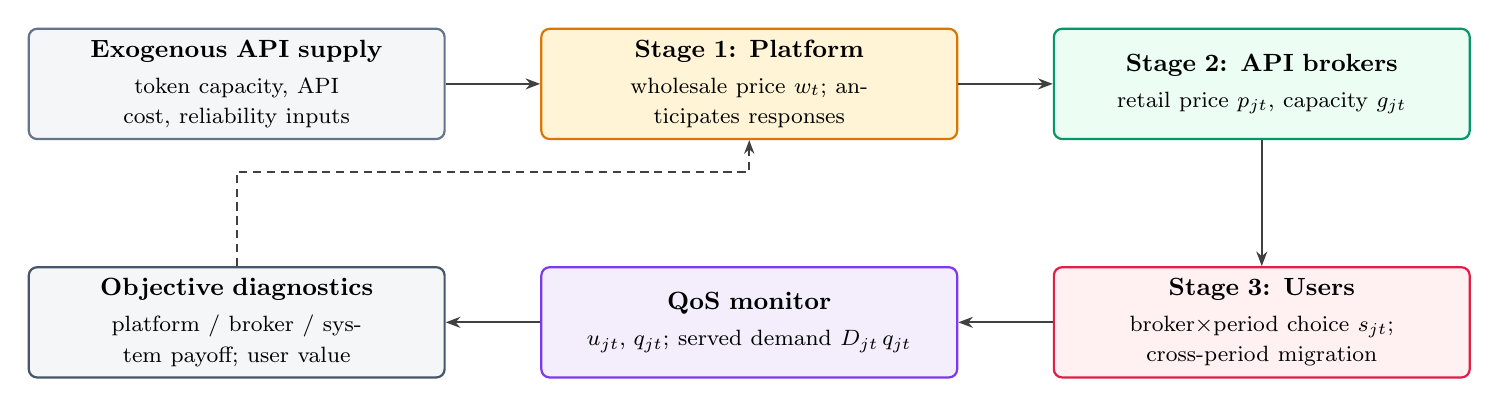
\begin{tikzpicture}[
    node distance=1.6cm and 1.2cm,
    block/.style 2 args={
        rectangle, draw=#1, fill=#2, rounded corners=3pt,
        text width=5.0cm, minimum height=1.4cm, align=center,
        line width=0.8pt, font=\small, inner sep=4pt,
    },
    smallblock/.style 2 args={
        rectangle, draw=#1, fill=#2, rounded corners=3pt,
        text width=4.8cm, minimum height=1.15cm, align=center,
        line width=0.8pt, font=\scriptsize, inner sep=3pt,
    },
    arrow/.style={-{Stealth[scale=0.8]}, line width=0.8pt, color=darkgray},
    dasharrow/.style={-{Stealth[scale=0.8]}, line width=0.7pt, color=darkgray, densely dashed},
    darkgray/.style={color=black!55},
]

% ── color definitions ──────────────────────────────
\definecolor{bgSupply} {HTML}{F4F6F8}
\definecolor{bdSupply} {HTML}{64748B}
\definecolor{bgPlat}   {HTML}{FFF4D6}
\definecolor{bdPlat}   {HTML}{D97706}
\definecolor{bgBroker} {HTML}{ECFDF3}
\definecolor{bdBroker} {HTML}{059669}
\definecolor{bgUser}   {HTML}{FFF1F2}
\definecolor{bdUser}   {HTML}{E11D48}
\definecolor{bgMonitor}{HTML}{F3EDFC}
\definecolor{bdMonitor}{HTML}{7C3AED}
\definecolor{bgRevenue}{HTML}{F4F6F8}
\definecolor{bdRevenue}{HTML}{475569}

% ── nodes ──────────────────────────────────────────
\node [block={bdSupply} {bgSupply}] (supply) {
    \textbf{Exogenous API supply}\\[2pt]
    {\footnotesize token capacity, API cost, reliability inputs}
};

\node [block={bdPlat} {bgPlat}, right=of supply] (plat) {
    \textbf{Stage 1: Platform}\\[2pt]
    {\footnotesize wholesale price $w_t$; anticipates responses}
};

\node [block={bdBroker} {bgBroker}, right=of plat] (broker) {
    \textbf{Stage 2: API brokers}\\[2pt]
    {\footnotesize retail price $p_{jt}$, capacity $g_{jt}$}
};

\node [block={bdUser} {bgUser}, below=of broker] (user) {
    \textbf{Stage 3: Users}\\[2pt]
    {\footnotesize broker$\times$period choice $s_{jt}$; cross-period migration}
};

\node [block={bdMonitor}{bgMonitor}, left=of user] (monitor) {
    \textbf{QoS monitor}\\[2pt]
    {\footnotesize $u_{jt},\, q_{jt}$; served demand $D_{jt}\,q_{jt}$}
};

\node [block={bdRevenue}{bgRevenue}, left=of monitor] (revenue) {
    \textbf{Objective diagnostics}\\[2pt]
    {\footnotesize platform / broker / system payoff; user value}
};

% ── arrows ─────────────────────────────────────────
\draw [arrow] (supply.east)  -- (plat.west);
\draw [arrow] (plat.east)    -- (broker.west);
\draw [arrow] (broker.south) -- (user.north);
\draw [arrow] (user.west)    -- (monitor.east);
\draw [arrow] (monitor.west) -- (revenue.east);

% Feedback loop
\draw [dasharrow] (revenue.north) -- ++(0,1.2) -| (plat.south);

\end{tikzpicture}
\end{document}
